\chapter{Praktischer Teil}
\label{sec:praktischerteil}
\begin{onehalfspace}
In diesem Teil der Arbeit werden zuerst die beiden Szenarien erläutert und daraufhin die Konzeption und Umsetzung derer in Python beschrieben.
\section{Szenarien}
\label{subsec:szenarien}
Für das generieren von Daten wurden zwei möglichst reale Szenarien ausgewählt. Zum einen das Szenario eines Bewährungsantrages, für welches 5 verschiedene Attribute und eine endgültige Bewertung mit stattgegeben oder nicht generiert werden. Zum anderen das zweite Szenario des social creditpoint system, für welches pro Person 7 Attribute zu generieren sind und eine numerische Bewertung zwischen 600 und 1400 creditpoints erstellt wird. Diese beiden Szenarien werden im folgenden genauer erläutert.
\subsection{Szenario 1}
\label{subsubsec:szenario1}
In Szenario 1 soll ein Bewährungsantrag einer Person Bewertet werden. Ein Antrag besteht dabei aus dem Namen der Person, dessen Geschlecht, Hautfarbe und den entscheidenden Attributen der laufenden Strafe in Jahre und der Härte des Vergehens. Basierend auf diesen Attributen soll ein Bewerter beurteilen, ob der Antrag genehmigt oder abgelehnt wird. Das Geschlecht wird in \glqq{}Männlich\grqq{} und \glqq{}Weiblich\grqq{} angegeben. Da zur Vereinfachung sich auf das biologische Geschlecht begrenzt wurde und aus diesem Grund die Genderdiversität für den Datengenerator au{\ss}envor gelassen wurde. Die Hautfarbe der Person wird als \glqq{}Schwarz\grqq{} oder \glqq{}Weiß\grqq{} festgehalten. Die noch laufende Strafe des Gefangenen wird in Jahren von als Ganzzahlen von 1-5 angegeben. Da hier definiert wird ein Bewährungsantrag kann erst ab maximal 5 Jahren noch offene Strafe gestellt werden. Die Härte des Vergehens wird einfachheitshalber in den Gruppen \glqq{}Leicht\grqq{}, \glqq{}Mittel\grqq{} oder \glqq{}Hart\grqq{} festgehalten. \newline
Für die Beurteilung des Antrags von dem Bewerter werden folgende Regeln definiert:
\begin{table}[!h]
    \centering
    \begin{tabular}{|l|l|l|}
    \hline
    \textbf{Attribut}   & \textbf{Positive Auswirkung} & \textbf{Negative Auswirkung} \\ \hline
    Laufende Strafe     & 1-3                          & 4-5                          \\ \hline
    Härte des Vergehens & Leicht, Mittel               & Hart                         \\ \hline
    \end{tabular}
\caption{Tabelle für die Auswirkung der Attributen von Szenario 1}
\label{table:1}
\end{table}\\
Das Geschlecht und die Hautfarbe werden hierbei nicht direkt aufgelistet, da diese in der Regel keine Auswirkung auf die Bewertung haben sollten. Diese können jedoch durch einen konkreten Bias Aussagekraft bekommen. Damit soll in den generierten Daten die gewünschte Verzerrung auf einen gewissen Wert gelegt werden können. In diesem Szenario sind die möglichen Werte, welche durch eine Verzerrung und damit einem menschlichem Vorurteil eines Bewerters beeinflusst werden können, das Geschlecht und die Hautfarbe. Die anderen beiden Attribute, welche in der Tabelle \ref*{table:1} aufgeführt sind, wirken sich durch ihre Ausprägungen positiv oder negativ auf die Bewertung des Antrages aus. So wirkt z.B. eine Härte des Vergehens vom Niveau Leicht sich eher für eine positive Bewertung des Antrages aus, als eine mittlere Härte. Dasselbe gilt auch für die Laufende Strafe. So kann ein Bewerter dann anhand dieser beiden Werte eine Tendenz erhalten und dann über die Gestattung des Antrages entscheiden.
\subsection{Szenario 2}
\label{subsubsec:szenario2}
Im zweiten Szenario wird das durch China populär gewordene sozial creditpoint System in einer lagenunabhängigen Version nachgebaut. Dafür werden Einträge zu Personen erstellt, nach welchen die Punktzahl der einzelnen Person zwischen 600 und 1400 Punkten bestimmt wird. Ein Eintrag zu einer Person beinhaltet die sieben in der folgenden Tabelle dargestellten Attribute mit den unterschiedlichen Ausprägungen.
\begin{table}[!h]
    \centering
    \begin{tabular}{|l|l|}
    \hline
    \textbf{Attribut}       & \textbf{Ausprägungen}                                                                                                \\ \hline
    Name                    & Beliebig                                                                                                             \\ \hline
    Alter                   & 20-79                                                                                                                \\ \hline
    Politische Orientierung & Links, Mitte, Rechts                                                                                                 \\ \hline
    Bildungsabschluss       & \begin{tabular}[c]{@{}l@{}}Ausbildung, Fachschulabschluss, \\ Bachelor, Master, Diplom, Promotion, ohne\end{tabular} \\ \hline
    Soziales                & 0-3                                                                                                                  \\ \hline
    Wohnlage                & \begin{tabular}[c]{@{}l@{}}Großstadt, Kleinstadt,\\ Vorort, Ländlich\end{tabular}                                    \\ \hline
    CO2-Fußabdruck          & 4-12                                                                                                                 \\ \hline
    \end{tabular}
\caption{Tabelle der Attribute und Auswirkungen von Szenario 2}
\label{table:2}
\end{table}
Die in Tabelle \ref*{table:2} aufgeführten Ausprägungen haben ähnlich wie zu Szenario 1 unterschiedlich starke Auswirkungen auf den am Ende bestimmten social Score. Einzig allein der Name und das Alter sollen keine direkte Auswirkung auf den social Score haben. Die anderen Attribute wirken sich je nach Auswirkung positiv durch eine Erhöhung des Scores oder negativ durch eine Verringerung des Scores aus.
Insgesamt werden so in diesem Szenario viele Einträge von Personen erstellt, welche alle unterschiedlichste Verteilungen der Ausprägungen besitzen und dadurch in der Bewertung einen individuellen social Score erzielen. Um nun eine gewünschte Verzerrung in die Daten zu bekommen können alle Attribute bis auf den Namen, welcher rein als Füllwert dient, durch eine Verzerrung beeinflusst werden. So können z.B. Personen zwischen 20-30 Jahre negativ verzerrt werden, da ein oder zwei Bewerter etwas gegen junge Leute haben und diesen aus ihrer Überzeugung einen schlechteren Score geben. In diesem Szenario ist somit eine hohe Variabilität geboten inwieweit eine Verzerrung in die Daten gebracht wird. Zudem kann auch eine Verzerrung über mehrere Attribute eingebracht werden, da ein Bewerter z.B. auch etwas gegen eine Rechte Politische Orientierung und ein schlechtes Soziales Engagement von 0 haben kann. 
\section{Konzeption}
\label{subsection:konzeption}
In diesem Kapitel wird die erarbeitete Konzeption für die Umsetzung der beiden im Kapitel \ref*{subsec:szenarien} aufgeführten Szenarien erläutert. Dabei wird in ein Grobkonzept zur allgemeinen Generierung der Daten und darauf in ein Feinkonzept für jedes Szenario unterteilt.
\subsection{Grobkonzept}
\label{subsubsec:grobkonzept}
Das Grobkonzept beinhaltet die Überlegungen, wie die Programme/Notebooks für die beiden Szenarien generell aufgebaut sein sollen. Der Ablauf der Programme von der Eingabe der Parameter bis hin zu den fertig generierten Daten wird in fünf Schritten durchgeführt. Der Ablauf der Schritte ist in folgendem Programmablaufplan dargestellt.\\
\begin{figure}[h]
    \centering
    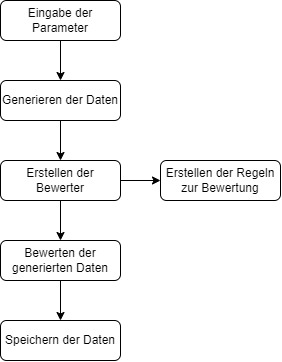
\includegraphics[width=6cm,height=8cm]{Diagramme/Grobkonzept_PAP.jpg}
    \caption{Programmablaufplan der fünf Hauptschritte zur Generierung der Daten}
    \label{fig:GrobkonzeptPAP}
\end{figure}\\
Die in der Abbildung \ref{fig:GrobkonzeptPAP} dargestellten Hauptschritte des Programmablaufs lauten: Parametereingabe, Generieren der Daten, Regeln aufstellen, Bewerten und Speichern der Daten. Im ersten Schritt der Parametereingabe, wird den Benutzenden die Möglichkeit gegeben die Parameter für die Generierung der Daten einzugeben, wie z.B. die Anzahl der Daten oder Bewertende welche generiert werden sollen. Im folge Schritt werden daraufhin die passende Anzahl an Daten für das jeweilige Szenario generiert. Dabei sollen die Daten möglichst an Verhältnissen aus der Realität angepasst und auf dieser Grundlage generiert werden. Es soll jedoch eine gewisse Zufälligkeit in der Generierung vorhanden sein, sodass bei mehrfach Generierung unterschiedliche Datensätze auf Basis der definierten Verteilungen entstehen. Nach Abschluss der Generierung wird der fertige Datensatz zwischengespeichert, um diesen später bewerten zu können. Für die Bewertung des Datensatzes muss im folgenden 3. Schritt die Regeln nach welchen bewertet wird aufgestellt werden. Dafür soll zuerst die in den Parametern gewünschte Anzahl an Bewertenden erstellt werden, da durch diese die Regeln erstellt werden. Unter den Erstellten Bewertenden müssen zudem noch die angegebene Anzahl an diskriminierenden Bewertenden in solche umgewandelt werden. Daraufhin können dann die Regeln für die Bewertenden erzeugt werden. Somit ist der 3. Schritt abgeschlossen und alle Vorbereitungen getroffen für die Bewertung. In der Bewertung bekommen die Bewertenden alle Anträge des Datensatzes vorgelegt, welche Sie basierend auf den Regeln bewerten. Die Bewertung des jeweiligen Antrages wird diesem in den Daten hinzugefügt. Damit kann zum letzten Prozess übergegangen werden. In diesem wird der Ursprungsdatensatz und der bewertete Datensatz abgespeichert und damit auch au{\ss}erhalb von dem Programm zugänglich gemacht.\\
Somit ist das Grobkonzept der Szenarien abgeschlossen und ein Grundgerüst konnte entworfen werden. Im weiteren kann nun auf die detaillierte Feinkonzeption der einzelnen Szenarien eingegangen werden.
\subsection{Feinkonzept}
\label{subsubsec:feinkonzept}
Die im Grobkonzept beschriebenen fünf Hauptschritte der Programme sind für beide Szenarien gleich. Jedoch unterscheiden sich die Schritte im Detail bei beiden Szenarien. Daher wird für jedes Szenario ein eigenes Feinkonzept zur Füllung des selben vorhanden Grundgerüst entwickelt.\\
\textbf{Parametereingabe}\\
Im ersten Schritt der Parametereingabe unterscheiden sich die Szenarien nicht, da beide einen Parameter für die gewünschte Diskriminierung, die Anzahl der Daten, die Anzahl der Bewertenden, die Anzahl der diskriminierenden Bewertenden und der stärke der Auswirkung von der Diskriminierung benötigen. Diese Parameter können von den Benutzenden in beiden Fällen in einer finalen Zelle editiert werden.\\
\textbf{Daten generieren}\\
In diesem Prozess unterscheiden sich beide Szenarien stark, da zum einen für das erste Szenario nur fünf anstelle von sieben Attribute bei Szenario 2 generiert werden müssen und zum anderen existieren deutlich weniger Verbindungen zwischen den Attributen in Szenario 1. Bei dem ersten Szenario basiert nur die Härte der Strafe und die Hautfarbe auf dem Geschlecht, dies bedeutet die Wahrscheinlichkeiten für diese Attribute soll dem Geschlecht entsprechend angepasst werden. So haben zum Beispiel weibliche Personen eine eher seltener eine Harte Strafe als männliche Personen. Alle anderen Attribute in diesem Szenario haben eine feste Wahrscheinlichkeitsverteilung. Damit sind die Zusammenhänge in diesem Szenario sehr klein gehalten und überschaubar.\\
In Szenario 2 müssen sieben Attribute generiert werden und es sollen deutlich mehr Verbindungen zwischen diesen existieren. Um diese verständlich darzustellen wurde ein Diagramm für das Feinkonzept entworfen, welches nachfolgend dargestellt ist.\\
\begin{figure}[h]
    \centering
    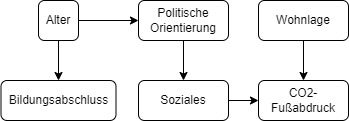
\includegraphics{Diagramme/Verbindung_der_Attribute_S2.jpg}
    \caption{Verbindungen zwischen den Attributen des zweiten Szenario}
    \label{fig:VerbindungenS2}
\end{figure}\\
In der Abbildung \ref{fig:VerbindungenS2} sind alle Attribute, bis auf das Attribut Name, des zweiten Szenario als abgerundete Rechtecke und die Verbindungen zwischen diesen mit Pfeilen dargestellt. Insgesamt existieren wie zu sehen fünf Verbindungen zwischen den Attributen. Diese sollen so aufgebaut werden, um möglichst Realitätsnahe Daten generieren zu können. Die Verbindung zwischen dem Alter und dem Bildungsabschluss existiert, da zum Beispiel die Wahrscheinlichkeit, dass eine Person mit 20 schon eine Promotion besitzt nicht so hoch ist wie bei einer Person im Alter von 50. Zudem hat das Alter einen Einfluss auf die Politische Orientierung einer Person, da junge Leute sicherlich andere Orientierungen haben als Personen im Alter von 50 zum Beispiel, siehe Aktionen wie \glqq{}FridaysforFuture\grqq{}. Durch die Politische Orientierung einer Person wird in diesem Fall auch mit einer Beeinflussung auf das soziale Verhalten gerechnet und es besteht daher hier auch eine Verbindung. Im Falle des CO2-Fußabdruck wird in dieser Arbeit mit einer Auswirkung der Wohnlage und einer Auswirkung des Sozialen gerechnet. Durch das Soziale und die Vorverbindung wird die Politische Orientierung und das Alter ebenfalls indirekt darauf mit ein Bezogen. Dies ist hier der Fall, da die Berechnung CO2-Fußabdruck sich aus vielen Faktoren zusammensetzt und daher auch dieser in diesem Szenario durch viel beeinflusst werden soll. Durch diese Zusammenhänge sollen dann möglichst realitätsnahe Daten entstehen.\\
Insgesamt für beide Szenarien müssen dann später bei der Umsetzung die Wahrscheinlichkeiten der Ausprägungen der Attribute, wo es möglich ist, durch Statistiken bestimmt werden und die Verbindungen dadurch ebenfalls bestätigt werden. Dies wird im Kapitel \ref{umsetzung} im Detail erläutert.\\
\textbf{Regeln aufstellen}\\
Im diesem Schritt werden zuerst bei beiden Szenarien die gewünschte Anzahl an Bewertenden erstellt, von welchen danach die Anzahl an diskriminierenden ausgewählt wird. In der folge können die Regeln für die zuvor als Objekte erstellte Bewertenden erstellt werden. Im Fall des ersten Szenarios werden zwei Listen mit Hilfe der unter Kapitel \ref{subsubsec:szenario1} gezeigten Tabelle erstellt. Eine Liste beinhaltet die in der Tabelle dargestellten Positiven Auswirkungen und die andere Liste beinhaltet die Negativen Auswirkungen. So haben die Objekte der Bewertenden ihre eigenen Listen an Regeln. Daher kann für die diskriminierenden Bewertenden in der Liste der Negativen Auswirkungen das zu diskriminierende Attribut hinzugefügt werden. So diskriminieren diese Bewertenden automatisch, da sie diese Regeln zur Überprüfung der Bewertung haben. Für das zweite Szenario sieht das Konzept hier etwas anders aus, da es hier nicht um eine Bewertung in genehmigt oder nicht geht, sondern um Punkte. Somit müssen die Regeln so erstellt werden, dass die Bewertenden eine Liste an allen Ausprägungen der Attributen haben und dazu eine passende Zuordnung mit wie vielen Punkten sich welche Ausprägung auf den Score auswirkt. Die Verzerrung wird in diesem Fall erst im nächsten Schritt der Bewertung betrachtet.\\
\textbf{Bewertung}\\
Folgend auf die erstellten Regeln können die Bewertenden nun die vorgelegten Einträge der Daten bewerten. Im ersten Szenario wird das ganze durch eine Wahrscheinlichkeitsverteilung durchgeführt. Zu Beginn jeder Bewertung steht es 50:50 für genehmigt oder nicht. Durch die erstellten Regel Listen können dann die Bewertenden die im Antrag aufgeführten Attribute abgleichen, ob diese sich positiv (also für eine Genehmigung) oder negativ auswirken. Nach dieser Bestimmung wird dann die Wahrscheinlichkeitsverteilung verschoben in positive oder negative Richtung. So kann am Ende wenn der Bewertende alle Attribute durch hat mit Hilfe der übrig gebliebenen Wahrscheinlichkeiten für positiv und negativ eine Entscheidung getroffen werden. Falls ein bewertendes Objekt diskriminieren sollte, hat dieses wie oben erläutert in seinen negativen Regeln die gewünschte Ausprägung enthalten, sodass diese sich dann auf die Entscheidung auswirkt. Für das zweite Szenario wird nicht mit einer Wahrscheinlichkeitsverteilung gearbeitet, sondern mit dem mittleren Wert des Scores als Startwert(1000). So können die Bewertenden von Attribut zu Attribut aus dem zu bewertenden Eintrag durchlaufen und entsprechend nach der Ausprägung den in Ihren eigenen Regeln definierte Wert dem Startwert hinzu addieren. Damit entsteht dann letztendlich der finale Score für den Eintrag. Für die Verzerrung wird das Attribut und die Ausprägung dessen welche verzerrt werden soll in jedem Eintrag gesucht. Falls die gewünschte Ausprägung vorhanden ist wird der Score dieses Eintrages um die in den Parametern eingegebene negative Auswirkung für die Verzerrung addiert.\\
Insgesamt werden bei beiden Szenarien die Einträge aus dem generierten Datensatz zufällig einem Bewertenden zur Bewertung zugeordnet. So ist eine zusätzliche Variabilität in der Verteilungen der Verzerrung gegeben.\\
\textbf{Speichern der Daten}\\
Zum Abschluss werden bei beiden Szenarien gleich die beiden Datensätze als CSV Datei gespeichert. Zum einen den ursprünglich generierten Datensatz und zum anderen auch der Datensatz mit der jeweiligen Bewertung enthalten. Durch eine CSV Datei können die Daten dann beliebig in anderen Programmen weiterverwendet werden.\\
Insgesamt ist damit die Konzeption abgeschlossen. Im Grobkonzept wurde ein Grundgerüst für die beiden Programme der Szenarien entworfen, welches auch für noch weitere Szenarien der Art verwendet werden kann. Im Feinkonzept wurde dann das Grundgerüst durch Inhalt der jeweiligen Szenarien gefüllt und das geplante im Detail beschrieben. So kann nun zur Umsetzung der beiden Programme als Notebooks übergegangen werden.
\section{Umsetzung}
\label{umsetzung}
Da die Programme als Notebooks in python umgesetzt sind, können die einzelnen, in der Konzeption dargestellten, Prozessschritte als Zellen verwirklicht werden. Nun wird die Umsetzung des ersten Szenarios beschrieben.\\
Im Programm für das erste Szenario, welches \glqq{}Szenario1.ipynb\grqq{} heißt, müssen zu aller erst in der ersten Zelle die benötigten Bibliotheken geladen werden.
\begin{figure}[h]
    \centering
    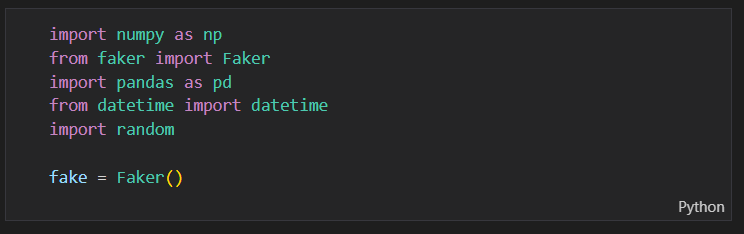
\includegraphics{Diagramme/Sz1_Cell1.PNG}
    \caption{Erste Zelle Code des Szenario1}
    \label{fig:Zelle1S1}
\end{figure}\\
In der Abbildung \ref{fig:Zelle1S1} ist die erste Zelle mit den Importen der Bibliotheken zu sehen. Die Bibliothek \glqq{}numpy\grqq{} wird für Zufallsauswahlen unter bestimmten Wahrscheinlichkeiten benötigt. \glqq{}faker\grqq{} ist eine Bibliothek für generierte Daten, so wird diese hier für das bestimmen zufälliger Namen verwendet. \glqq{}pandas\grqq{} bietet sogenannte Dataframes in welchen die Daten gespeichert werden und durch pandas auch in eine CSV Datei geschrieben werden können. Die letzte Bibliothek \glqq{}random\grqq{} ist ebenfalls wie \glqq{}numpy\grqq{} für das generieren von Zufallswerten zuständig. Zum Schluss wird in der Zelle noch eine Instanz der Faker Klasse erstellt, welches zur Verwendung der Bibliothek benötigt wird.\\
In der nächsten Zelle ist die Methode \glqq{}create\_fake\_data\grqq{} zur Generierung der Daten umgesetzt. Diese Methode bekommt die beiden Parameter num und seed übergeben. Der Parameter seed wird zu Beginn verwendet um den Startwert der Faker Instanz und von \glqq{}numpy\grqq{} zu setzen. Dadurch wird es ermöglicht, mit unterschiedlichen Startwerten, eine nahezu \glqq{}echte\grqq{}Zufallszahl zu generieren. Bei gleichbleibendem Startwert und gleicher Methode würde der Code immer die gleiche Zufallszahlen bestimmen. Zum Beispiel wenn drei Zahlen von 0-10 generiert werden sollen, werden bei gleichem Startwert immer die drei selben Zahlen generiert. Variiert der Startwert jedoch, werden jedes Mal unterschiedliche Zahlen generiert und eine ausreichende Variabilität erreicht. Als nächstes wird mit einer Schleife über die im Parameter num angegebene Zahl iteriert. In jedem Schleifendurchlauf wird ein Eintrag für den Datensatz generiert. Somit ist num die Größe des gewünschten Datensatzes. In diesem Szenario müssen somit in jedem Durchlauf ein Wert für die Attribute Name, Geschlecht, Härte der Strafe, Hautfarbe und Laufende Strafe ermittelt werden. Der Name in jedem Eintrag wird durch die Faker Instanz generiert. Dafür wird je nach Geschlecht die Methode zum generieren eines weiblichen oder männlichen Namen aufgerufen. Die Attribute Geschlecht, Härte der Strafe und Hautfarbe müssen nach bestimmten Wahrscheinlichkeiten berechnet werden. Dies wird für jedes dieser Attribute wie folgend ausgeführt:\\
\textbf{Geschlecht}\\
Formel zur Berechnung der Wahrscheinlichkeiten für \ac{M} und \ac{W}:\\
Gegeben: Gesamt = Gesamt Zahl der Gefangenen\\
\begin{equation}
    W/M\% = \frac{W/M}{Gesamt}\label{eq:Sz1Mänlich}
\end{equation}
\begin{table}[h]
    \centering
    \begin{tabular}{|c|c|c|}
    \hline
    \textbf{Ausprägungen} & \textbf{Berechnung} & \textbf{Wahrscheinlichkeit} \\ \hline
    Weiblich              &\rule{0pt}{18pt} $\frac{105.000}{1.439.800}$  & 7,3\% \\[8pt] \hline
    Männlich              & \rule{0pt}{18pt}$\frac{1.334.800}{1.439.800}$     & 92,7\%  \\[8pt] \hline
    \end{tabular}
\caption{Tabelle zur Bestimmung der Wahrscheinlichkeiten für das Geschlecht}
\label{table:3}
\end{table}
Das Geschlecht für eine Person wird nach den in der Tabelle \ref{table:3} berechneten Wahrscheinlichkeiten bestimmt. Die hier berechneten Wahrscheinlichkeiten ergeben sich aus den Gefängniszahlen von 2017 der USA, welche in einem Beitrag des U.S. Department of Justice im April 2019 veröffentlicht wurden. Die Zahlen wurden hierbei aus der \glqq{}Table 8\grqq{} des Papers entnommen und zur Berechnung nach der oben aufgeführten Formel verwendet.\cite[S. 17]{Bronson2017}\\
Die daraus entstehenden Wahrscheinlichkeiten werden wie in der folgenden Abbildung\ref{fig:GeschlechtscodeS1} zur Bestimmung des Geschlechts mit Hilfe der \glqq{}numpy\grqq{} Bibliothek verwendet.
\begin{figure}[h]
    \centering
    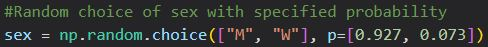
\includegraphics{Diagramme/Sz1_GeschlechtsCode.JPG}
    \caption{Codezeile zur Bestimmung des Geschlechts einer Person}
    \label{fig:GeschlechtscodeS1}
\end{figure}\\
In der Zeile Code werden zuerst die möglichen Ausprägungen als Strings in einem Array angegeben und dann die dazugehörigen Wahrscheinlichkeiten nach welchen eine Ausprägung bestimmt werden soll.\\
\textbf{Härte der Strafe}\\
Für die Bestimmung einer Ausprägung der Härte der Strafe, ist die Berechnung der Wahrscheinlichkeiten und die letztendliche Auswahl etwas komplexer. Da wie in der Konzeption geplant die Härte der Strafe vom Geschlecht einer Person abhängig ist. Daher ist es nicht möglich eine einfache Formel zur Berechnung aufzustellen, sondern es muss aus der Datenquelle erörtert werden wie sich die Wahrscheinlichkeiten verteilen. Die Verteilung der Wahrscheinlichkeiten ist in der folgenden Tabelle dargestellt.\\
\begin{table}[h]
    \centering
    \begin{tabular}{|l|l|l|}
    \hline
    \textbf{Ausprägungen} & \textbf{Weiblich} & \textbf{Männlich} \\ \hline
    Leicht                & 36,1\%            & 26,6\%            \\ \hline
    Mittel                & 26,4\%            & 16,9\%            \\ \hline
    Hart                  & 37,5\%            & 56,5\%            \\ \hline
    \end{tabular}
\caption{Tabelle der Wahrscheinlichkeiten für die Härte der Strafe nach Geschlecht}
\label{table:4}
\end{table}\\
Die in Tabelle \ref{table:4} gezeigten Wahrscheinlichkeiten ergeben sich aus dem Beitrag des U.S. Department of Justice vom April 2019. In diesem ist in \glqq{}Table 12\grqq{} eine prozentuale Verteilung von den Strafgruppen Gewalttätig, Eigentum, Drogen, Öffentliche Ordnung und Sonstige über die Geschlechter \ac{W} und \ac{M} aus dem Dezember 2016 aufgelistet. Dabei sind die Strafen nach den schwersten Delikten absteigend aufgeführt. Somit wird diese Verteilung auf die in der Konzeption definierten Ausprägungen Leicht, Mittel und Hart verteilt. So wird der Prozentsatz der gewalttätigen Strafen Hart zugeordnet, die Eigentumsstrafen Mittel zugeordnet und die Drogen, Öffentliche Ordnung und Sonstigen Strafen Leicht zugeordnet. Dadurch ergeben sich auf Grundlage der Zahlen aus den USA die Wahrscheinlichkeiten in der Tabelle \ref{table:4}.\cite[S. 21]{Bronson2017}\\
Um die Bestimmung der Härte der Strafe nun durchzuführen, wird der selbe Code wie in Abbildung \ref{fig:GeschlechtscodeS1} gezeigt auf dieses Attribut angepasst und im Verbund mit einer if Abfrage zur Überprüfung des Geschlechts umgesetzt. So wird entsprechend dem Geschlecht einer Person nach den dazu passenden Wahrscheinlichkeiten die Härte der Strafe zufällig ausgewählt.\\
\textbf{Hautfarbe}\\
Formel zur Berechnung der Hautfarbe basierend auf dem Vorwissen des Geschlechtes:\\
Gegeben: Gesamt \ac{W}/\ac{M} = Anzahl an Weißen und Schwarzen Gefangenen pro (G)Geschlecht = S(Schwarz) + Wi(Weiß)\\
\begin{equation}
    S/Wi\% = \frac{S/Wi}{Gesamt \ac{W}/\ac{M}}\label{eq:Sz1Hautfarbe}
\end{equation}

\begin{table}[h]
    \centering
    \begin{tabular}{|c|c|c|}
    \hline
    \textbf{Ausprägungen} & \textbf{Berechnung} & \textbf{Wahrscheinlichkeit} \\ \hline
    Schwarz              &\rule{0pt}{28pt} $
        S\%= 
    \begin{cases}
        \frac{456.300}{843.700}\quad |&\text{Geschlecht: M}\\
        \frac{19.600}{68.700} \quad | &\text{Geschlecht: W}
    \end{cases}$ & \(\displaystyle S\%=
    \begin{cases}
    54,1\%\quad | & \text{Geschlecht: M} \\
    28,5\%\quad| & \text{Geschlecht: W}
    \end{cases} \) \\[22pt] \hline
    Weiß              &\rule{0pt}{28pt} $
        Wi\%= 
    \begin{cases}
        \frac{387.400}{843.700}\quad |& \text{Geschlecht: M}\\
        \frac{49.100}{68.700} \quad |&\text{Geschlecht: W}
    \end{cases}$ & \(\displaystyle Wi\%=
    \begin{cases}
    45,9\%\quad | & \text{Geschlecht: M} \\
    71,5\%\quad | & \text{Geschlecht: W}
    \end{cases} \) \\[22pt] \hline
    \end{tabular}
\caption{Tabelle zur Bestimmung der Wahrscheinlichkeiten für die Hautfarbe unter Berücksichtigung des Geschlechts}
\label{table:5}
\end{table}
Die in der Tabelle \ref{table:5} dargestellten Berechnungen und daraus resultierenden Wahrscheinlichkeiten beruhen erneut auf der Veröffentlichung vom U.S. Department of Justice. In dieser sind in \glqq{}Table 8\grqq{} die Gefangenen nach Geschlecht und ethischen Gruppen aufgeteilt. Zur Vereinfachung wurden für die Hautfarbe jedoch nur zwischen Schwarz und Weiß unterschieden. Dabei werden Ethnien bewusst nicht gesondert berücksichtigt. Somit sind lediglich die Zahlen für die Anzahl an der Gruppe Schwarz und Weiß nach Geschlecht Männlich Weiblich von Interesse. Um daraus Prozentwerte zu bilden, nach welchen dann eine Person entweder die Hautfarbe Schwarz oder Weiß bekommt, wurde die oben gezeigte Formel aufgestellt. Für die Formel wird zuerst zum einen die Gesamtheit an Schwarzen sowie Weißen männlichen Personen und zum anderen die Gesamtheit am Schwarzen sowie Weißen weiblichen Personen gebildet. Daraufhin können basierend auf diesen Gesamtwerten die Wahrscheinlichkeitsverteilungen für Männlich und Schwarz, Männlich und Weiß, Weiblich und Schwarz, Weiblich und Weiß anhand der Formel berechnet werden.\\
Damit diese Wahrscheinlichkeiten bei der Bestimmung angewendet werden können wird wie schon bei der Härte der Strafe, der Code aus Abbildung \ref{fig:GeschlechtscodeS1} durch eine if Abfrage erweitert und an dieses Attribut angepasst.\\
Als letztes Attribut wird noch eine Ausprägung für die Länge der Strafe bestimmt. Hierfür wird mit der \glqq{}numpy\grqq{} Bibliothek eine zufällige Ganzzahl zwischen eins und fünf ausgewählt.\\
Um einen Schleifendurchlauf abzuschließen werden die durch Wahrscheinlichkeiten bestimmten Werte zusammen als ein Dictionary als neuen Eintrag in ein Array mit der Zuordnung(Attribut:Ausprägung) hinzugefügt. Damit ist ein Schleifendurchlauf abgeschlossen und der nächste kann beginnen. Wenn die Schleife fertig ist, wird das volle Array mit den gespeicherten Einträgen aus der Methode zum Datengenerieren zurückgegeben und diese ist damit auch vollends durchgeführt.\\
Als nächsten, aus der Konzeption definierten Prozessschritt nach dem generieren der Daten, wird das aufstellen der Regeln umgesetzt. Hierfür wird die Methode \glqq{}create\_Rules\grqq{} mit den Parametern\glqq{}request\_values, request\_bias, bias\grqq{} implementiert. Der Parameter \glqq{}request\_values\grqq{} ist ein Dictionary mit den Keys an den für die Bewertung relevanten Attributen und den dazugehörigen Ausprägungen in einem Array als Value. In diesem Fall sind es wie in der Konzeption definiert die Attribute Härte der Strafe und Laufende Strafe, welche wie in der folgenden Abbildung \ref{fig:RequestValues} im Dictionary angegeben werden.\\
\begin{figure}[h]
    \centering
    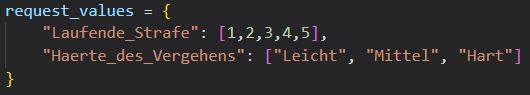
\includegraphics{Diagramme/Sz1_RequestValues.JPG}
    \caption{Codezeilen zum Erstellen eines Dictionary mit den zur Bewertung relevanten Attributen}
    \label{fig:RequestValues}
\end{figure}\\
Der Parameter \glqq{}request\_bias\grqq{} ist genau gleich aufgebaut, beinhaltet jedoch die Attribute Geschlecht und Hautfarbe und deren Ausprägung. Dieser gibt die Liste der durch Verzerrung beeinflussbaren Attribute an. Der letzte Parameter \glqq{}bias\grqq{} gibt die gewünschte Verzerrung ebenfalls wie die anderen Parameter an. 
In der Methode werden vier Rückgabewerte als Dictionaries generiert. Eine Dictionary für die Regeln der positiven Auswirkung, eines für die negative Auswirkung und nochmals die selben zwei Listen nochmals ergänzt durch die gewünschte Verzerrung. 
\begin{figure}[h]
    \centering
    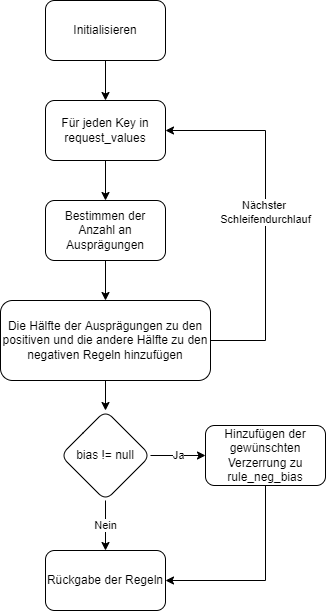
\includegraphics[width=8cm,height=14cm]{Diagramme/Sz1_Regeln.drawio.png}
    \caption{Programmablaufplan zur Generierung der Regeln von Szenario 1}
    \label{fig:Sz1Regeln}
\end{figure}\\
In Abbildung \ref{fig:Sz1Regeln} ist der Ablauf der Methode als Programmablaufplan skizziert. Zu Beginn werden die vier Dictionaries, in welchen die Regeln gespeichert werden, initialisiert. Daraufhin wird eine Schleife durch alle Keys des \glqq{}request\_values\grqq{} Dictionary durchlaufen. Darin werden als erstes die Anzahl an Ausprägungen des in diesem Durchlauf ausgewählten Attributes gezählt. Nach dem die Anzahl an Ausprägungen klar ist, kann die Mitte bestimmt werden. Anhand der Mitte werden die Ausprägungen unterhalb und gleich der Mitte dem Dictionary der negativen Regeln hinzugefügt und die restlichen oberhalb der Mitte dem Dictionary der positiven Regeln. Wenn dies vollbracht ist, ist der erste Durchlauf beendet und es kann mit dem nächsten weiter gemacht werden. 

NUN WEITER MIT RÜCKGABE WERTE UND DANN BESCHREIBUNG WIE LÄUFT METHODE AB WAS PASSIERT STÜCK FÜR STÜCK.
\newpage
\section{Datenauswertung}
\label{datenauswerung}
\section{Evaluation der Ergebnisse}
\label{evaluation}
\end{onehalfspace}